\begin{figure}[h]
    \centering
    \begin{tikzpicture}
        % Das Bild einfügen
        \node[anchor=south west, inner sep=0] (image) at (-1,0) 
              {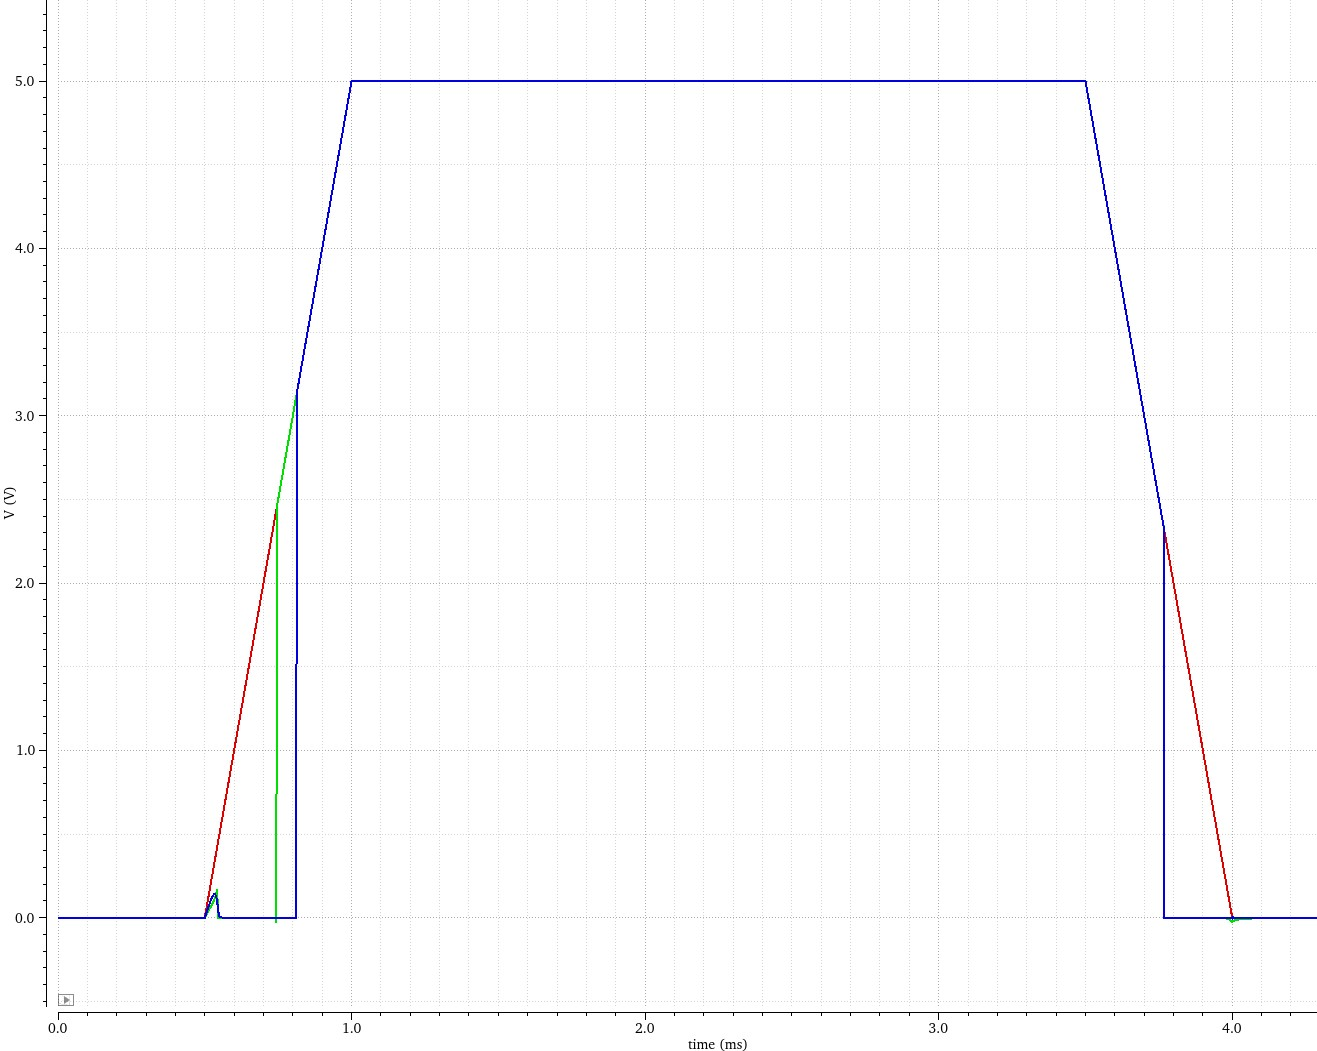
\includegraphics[width=0.8\textwidth]{figures/CD/waveform_standard.jpg}};

        % Legende hinzufügen
        \begin{scope}[shift={(0,-1)}]  % Position der Legende anpassen
            \draw[white] (0,0) rectangle (3.2,1.8); % Hintergrund für die Legende
            \node[anchor=west] at (-2,0.5) {\footnotesize\textcolor{red}{\textbf{---}} Betriebsspannung ($V_{DD}$)};
            \node[anchor=west] at (2,0.5) {\footnotesize\textcolor{green}{\textbf{---}} Komparatorausgang ($V_{comp}$)};
            \node[anchor=west] at (6.5,0.5) {\footnotesize\textcolor{blue}{\textbf{---}} Ausgang PoR-Schaltung ($V_{out}$)};
        \end{scope}
    \end{tikzpicture}
    \caption[Spannungsverläufe der Power-on-Reset-Schaltung]{: Spannungsverläufe der Power-on-Reset-Schaltung}
    \label{fig:por_waveform}
\end{figure}